\chapter{Volume Rendering}
\label{cap:vis_vol}

For volume rendering models, InVesalius employs a technique known as raycasting. In summary, raycasting is it a technique to simulate the trace a beam of light toward the object for each screen pixel. The pixel color is based on the color and transparence of each voxel intercepted by the light beam.

InVesalius there are several pre-defined patterns (presets) to display specific tissue types or different types of exam (tomographic contrast, for example).

To access this feature, simply click the shortcut shown in figure~\ref{fig:volume_raycasting_origina} in the lower right corner of the screen (next to the display window surfaces) and select one of the available standards.

To turn off the volume rendering, click again on the path indicated by the figure~\ref{fig:volume_raycasting_origina} and select the \textbf{Disabled} option.

\begin{figure}[!htb]
\centering
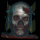
\includegraphics[scale=0.4]{volume_raycasting_origina}
\caption{Shortcut to volume visualization}
\label{fig:volume_raycasting_origina}
\end{figure}

\section{Viewing Standards}

There are several predefined viewing patterns. Some examples are illustrated in the following figures. 

\begin{figure}[!htb]
\centering
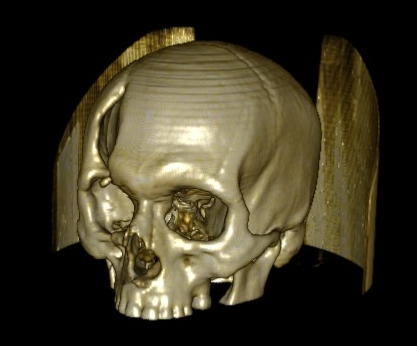
\includegraphics[scale=0.68]{brilhante_I}
\caption{Bright}
\label{fig:brilhante_I}
\end{figure}

\begin{figure}[!htb]
\centering 
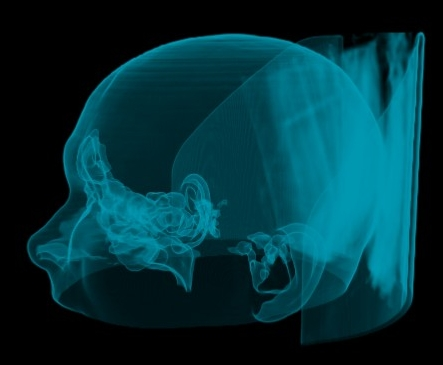
\includegraphics[scale=0.65]{vias_aereas_II}
\caption{Airway II}
\label{fig:vias_aereas_II} 
\end{figure}

\begin{figure}[!htb]
\centering
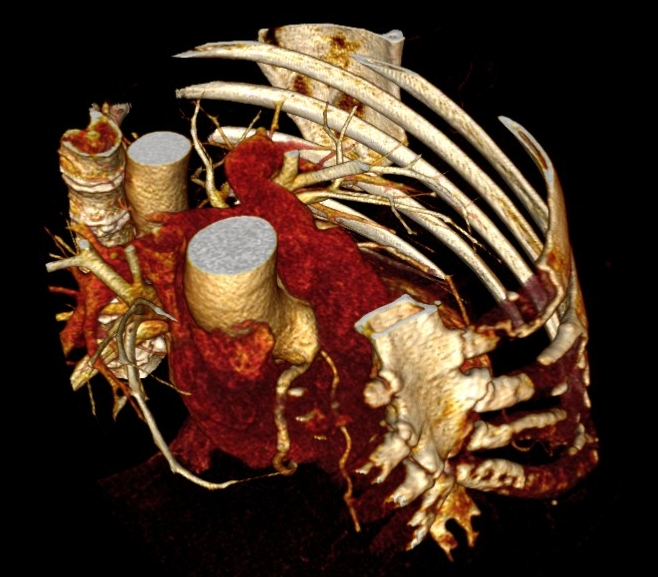
\includegraphics[scale=0.42]{contraste_medio}
\caption{Contrast Medium}
\label{fig:contraste_medio}
\end{figure}

\begin{figure}[!htb]
\centering
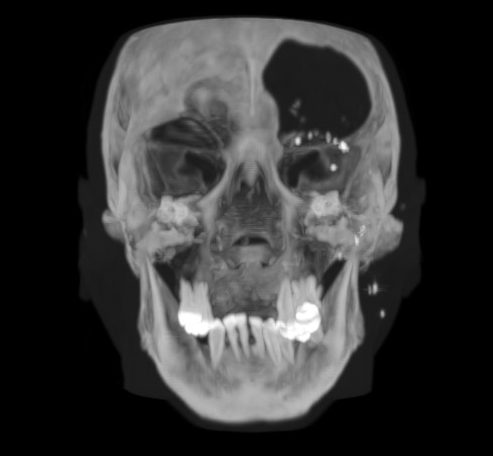
\includegraphics[scale=0.55]{MIP}
\caption{MIP}
\label{fig:MIP}
\end{figure}


\newpage


\section{Standard Customization}

Some patterns can be personalized (and customized). See figure~\ref{fig:customize_1}, which is exhibiting a pattern and some graphical controls adjustment. With these features, It is possible to change the color of a given structure and its opacity, determining if and how it will be displayed.

\begin{figure}[!htb]
\centering
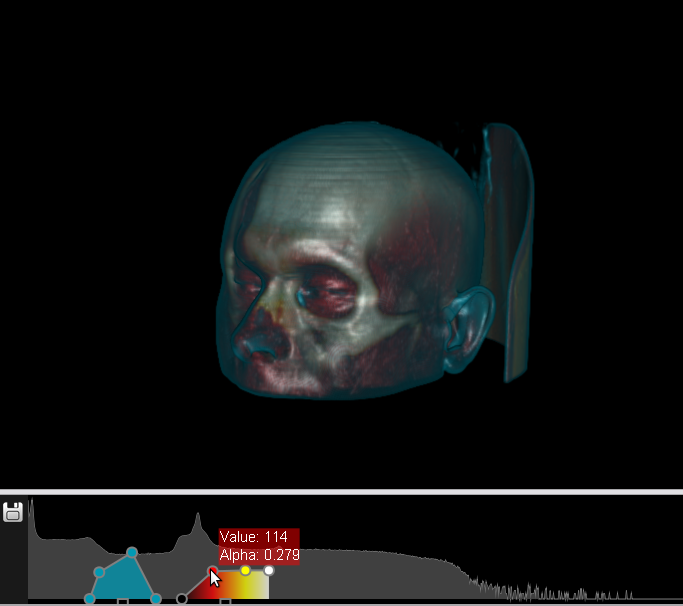
\includegraphics[scale=0.6]{customize_1}
\caption{Settings for the display pattern Soft Skin + II}
\label{fig:customize_1}
\end{figure}


\newpage

To hide a structure, you must use the control setting chart keeping low the opacity of the corresponding region. In the example in figure~\ref{fig:customize_1} for example, suppose you want to hide the muscular part, which appears in red. To do this, one can simply position the pointer over the point in red and using the left mouse button, drag the point down in order to reduce the opacity (which is equivalent to increasing transparency). Figure~\ref{fig:customize_2} illustrates the result.

Note: The Alpha value indicates the opacity of the color and the value Value, the color intensity of the pixel.

\begin{figure}[!htb]
\centering
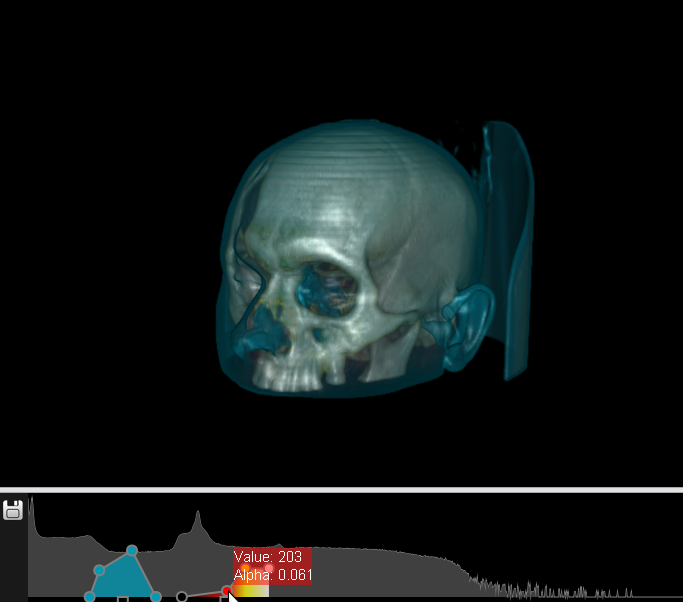
\includegraphics[scale=0.6]{customize_2}
\caption{Display Standard Soft Skin + II changed}
\label{fig:customize_2}
\end{figure}


\newpage


It can remove or add points on the graph control setting. For removing, simply click with the right mouse button on the point. For adding a new point, click the left button on the line
graph. One can also save the resulting pattern by clicking the shortcut.  Figure~\ref{fig:save_preset} illustrates.

\begin{figure}[!htb]
\centering

\includegraphics[scale=0.6]{save_preset}
\caption{Shortcut to save standard}
\label{fig:save_preset}
\end{figure}
 
To save the pattern, InVesalius displays a window like the one in figure~\ref{fig:save_window_preset}.
Enter a name for the custom pattern and \textbf{click OK} button. The saved pattern will be available with the other the next time the software is opened.

\begin{figure}[!htb]
\centering
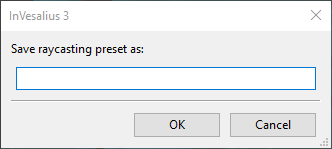
\includegraphics[scale=0.7]{save_window_preset_en.png}
\caption{Window to save name of pattern.}
\label{fig:save_window_preset}
\end{figure}

\section{Standard Customization with Brightness and Contrast}

You can customize a pattern without using the graphical control setting, which is presented in the previous section. This is done through the control \textbf{brightness and contrast} which is present in the toolbar. To activate the control, click the shortcut shown in figure~\ref{fig:tool_contrast_original_vol}.

\begin{figure}[!htb]
\centering

\includegraphics[scale=0.6]{tool_contrast_original}
\caption{Shortcut to Brightness and Contrast}
\label{fig:tool_contrast_original_vol}
\end{figure}

Enable the control by dragging the mouse, with the left button pressed on the volume window, this can change the values of the window width and window level. The procedure is the same as the slices applied to 2D, which can be seen in section~\ref{sec:ww_wl}. Dragging the mouse in the horizontal direction changes  the window level value. To the left, it decreases its window value, and for the right, it increases its window value. Dragging the mouse in the vertical direction changes the value of window width. If dragged down, the value is diminished and, dragging upwards increases its value.

Manipulating these values can be useful for different viewing results. For example, to add tissue to the display, \textbf{drag} the mouse diagonally with \textbf{left button} pressed from the lower right to the upper left corner of the preview window. To remove tissue visualization, do the opposite, (i.e \textbf{drag} the mouse diagonally from top left to bottom right with \textbf{left button} presseds.). See figure~\ref{fig:raycasting_add}.

\begin{figure}[!htb]
  \centering
  \subfloat[Bone]{\label{fig:raycasting_add_1}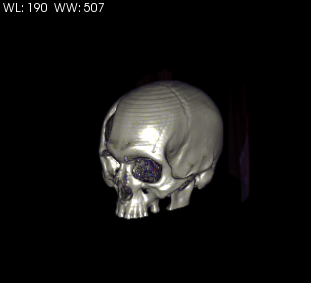
\includegraphics[width=0.33\textwidth]{raycasting_add_1}}                
  \hfill
  \subfloat[Muscle]{\label{fig:raycasting_add_2}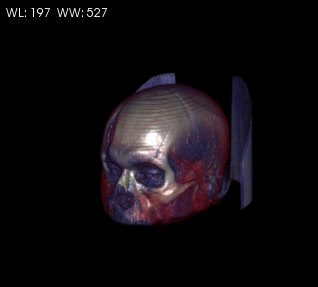
\includegraphics[width=0.333\textwidth]{raycasting_add_2}}	
  \hfill  
  \subfloat[Skin]{\label{fig:raycasting_add_3}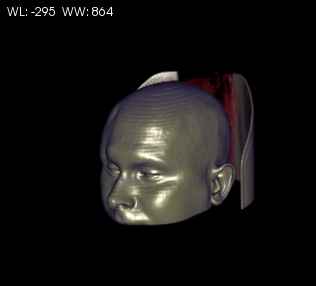
\includegraphics[width=0.332\textwidth]{raycasting_add_3}}
  \caption{Tissue Addition}
  \label{fig:raycasting_add}
\end{figure}

\newpage


\section{Cut}

In volume rendering, the cut is used to view a region of the internal volume. InVesalius has a cut for tool for this based on a reference plane. With a volume pattern selected, click \textbf{Tools}, and then click \textbf{Cut plane} (figure~\ref{fig:activate_cut_plane}).

\begin{figure}[!htb]
\centering
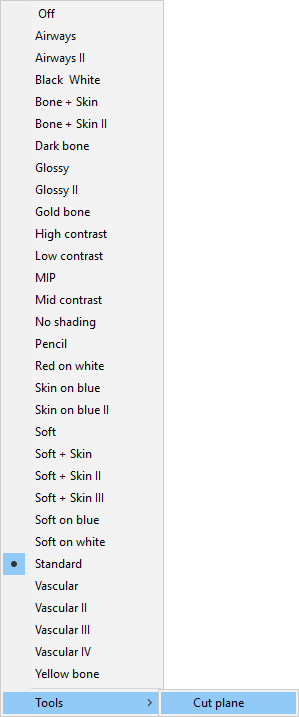
\includegraphics[scale=0.6]{activate_cut_plane_en.png}
\caption{Enabling plan to cut}
\label{fig:activate_cut_plane}
\end{figure}

A plan of representation for cutting appears next to the volume. To make the cut, hold the \textbf{left} mouse button on the plane and \textbf{drag} the mouse. To rotate the plan, hold the \textbf{left} mouse button pressed on its edge and move the mouse in the desired direction. See an example in figure~\ref{fig:cutted_image}.

\begin{figure}[!htb]
\centering
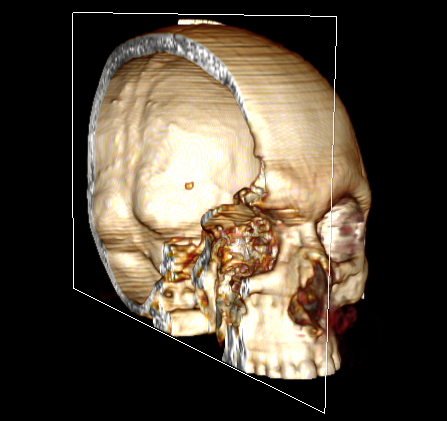
\includegraphics[scale=0.6]{cutted_image}
\caption{Image with clipping plane}
\label{fig:cutted_image}
\end{figure}

To disable the cut feature, click \textbf{Tools} and then again \textbf{Cut plan} (figure~\ref{fig:cutted_image}).